\documentclass[12pt]{article}
\usepackage{xr,geometry,fancyhdr,hyperref,ifpdf,amsmath,rcs}
\usepackage{color,lastpage,longtable,Ventry,url,paunits,shortcuts,smallsec,float}
\geometry{letterpaper,top=50pt,hmargin={20mm,20mm},headheight=15pt} 

\pagestyle{fancy} 

\RCS $Revision: 1.1 $
\RCS $Date: 2002/01/11 03:49:21 $

\fancypagestyle{first}{
\lhead{\textbf{A405: Pressure - volume carnot cycle review}}
\rhead{p.~\thepage/\pageref{LastPage}}
\lfoot{} 
\cfoot{} 
\rfoot{}
}

\ifpdf
    \usepackage[pdftex]{graphicx} 
    \usepackage{hyperref}
    \pdfcompresslevel=0
    \DeclareGraphicsExtensions{.pdf,.jpg,.mps,.png}
\else
    \usepackage{hyperref}
    \usepackage[dvips]{graphicx}
    \DeclareGraphicsRule{.eps.gz}{eps}{.eps.bb}{`gzip -d #1}
    \DeclareGraphicsExtensions{.eps,.eps.gz}
\fi
\externaldocument[lec1,]{lec1}
\externaldocument[lec2,]{lec2}
\externaldocument[lec3,]{lec3}

\begin{document}
\pagestyle{first}



\begin{itemize}

\item \textbf{Review -- Carnot cycle}:  To examine the thermodynamic efficiency of the atmosphere it's useful
to take as a reference the Carnot cycle.  First review how to draw an isotherm and an adiabat
on a $p, \alpha$ diagram:

\begin{itemize}
\item \textit{istotherm}:  $p \alpha \propto T = constant$
\item \textit{adiabat} (see problem set 1): $p \alpha^\gamma = constant$
\end{itemize}

\begin{figure}[htbp]
 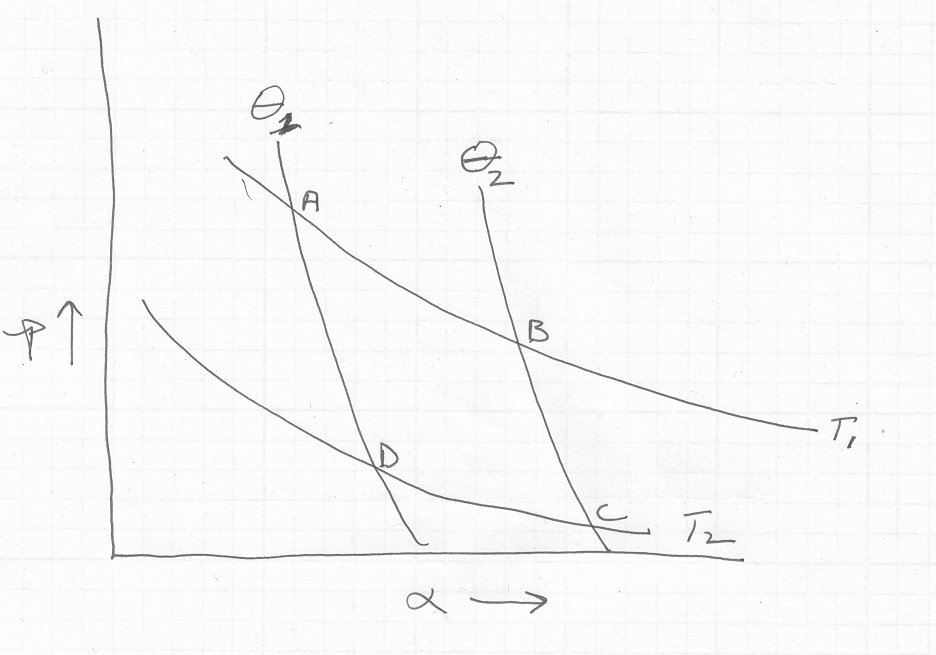
\includegraphics[width=6in]{carnot_pic.png}  
  \caption{Carnot cycle:two adiabats, two isotherms}
  \label{fig:carnot}
\end{figure}


\item As Figure~\ref{fig:carnot} indicates, there are four steps:

\begin{enumerate}
\item isothermal expansion
\par
$du=0$, $w dt =q dt$, $(p_A,\ \alpha_A\ T_1) \rightarrow (p_B,\ \alpha_B,\ T_1)$
\par
work done by system: 
\begin{equation}
  \label{eq:s1work}
\Delta w = \int p d \alpha = \int \frac{T_1}{\alpha} R_d d\alpha = T_1 R_d \log \frac{\alpha_B}{\alpha_A} > 0
\end{equation}
\par
so the system is heated, expands and does work.


\item adiabatic expansion
\par
$q dt=0$, $(p_B,\ \alpha_B\ T_1) \rightarrow (p_C,\ \alpha_C,\ T_2)$

\begin{eqnarray}
  \label{eq:s2work}
q dt &=& du + p d\alpha = cv dT + p d\alpha\\
\int p d\alpha &=& w dt = -du = -c_v (T_2 - T_1) > 0
\end{eqnarray}
work is done by system


\item isothermal compression
\par
$du=0$, $w dt = q dt$, $(p_C,\ \alpha_C\ T_2) \rightarrow (p_D,\ \alpha_D,\ T_2)$
\par
work done by air: 
\begin{equation}
  \label{eq:s3work}
\Delta w = \int p d \alpha = \int \frac{T_2}{\alpha} R_d d\alpha = T_2 R_d \log \frac{\alpha_D}{\alpha_C} < 0
\end{equation}
\par
system is cooled and work is done on system


\item adiabatic compression
\par
$q dt =0$, $(p_D,\ \alpha_D\ T_2) \rightarrow (p_A,\ \alpha_A,\ T_1)$

\begin{equation}
  \label{eq:s4work}
w dt = -du = -c_v (T_2 - T_1) < 0
\end{equation}
\par
work done on system.

\end{enumerate}

So heat is extracted from the reservoir at temperature $T_A$ (Congo) and returned to the
reservoir at temperature $T_B$ (Nova Scotia).


\item  Over the cycle $\oint du$ = $u_f$ - $u_i$ =0, since $u$ is a state variable and the
system returns to temperature $T_A$.  But this is not true for the integrated work
over the cycle.

\begin{equation}
  \label{eq:work}
  \oint w dt = T_1 R_d \log (\alpha_B/\alpha_A) + c_v (T_1 - T_2) - T_2 R_d \log (\alpha_C/\alpha_D) - c_v(T_1 - T_2)
\end{equation}

Note that we also have the following relationships for the isotherms and adiabats:

\begin{subequations}
\begin{eqnarray}
  \label{eq:isoadia}
  (isotherms):\ p_A \alpha_A &=&p_B \alpha_B\\ 
             \ p_C \alpha_C &=&p_D \alpha_D\\
  (adiabats):\ p_B \alpha_B^\gamma &=&p_C \alpha_C^\gamma\\ 
             \ p_D \alpha_D^\gamma &=&p_A \alpha_A^\gamma
\end{eqnarray}
\end{subequations}


\item Multiply these 4 equations together and divide by $p_A p_B p_C p_D$ to get:

  \begin{equation}
    \label{eq:alpha}
     \alpha_A \alpha_B^\gamma \alpha_C \alpha_D^\gamma = \alpha_B \alpha_C^\gamma \alpha_D \alpha_A^\gamma
  \end{equation}
Next divide by $\alpha_A^\gamma \alpha_B^\gamma \alpha_C^\gamma \alpha_D^\gamma$ to get:

\begin{equation}
  \label{eq:alpha2}
     \alpha_A^{(1-\gamma)} \alpha_C^{(1-\gamma)} =  \alpha_B^{(1-\gamma)} \alpha_D^{(1-\gamma)}
\end{equation}
Which reduces to

\begin{equation}
  \label{eq:alpha3}
  \alpha_B/\alpha_A = \alpha_C / \alpha_D
\end{equation}



\item Now go back to the first law:  define $\Delta q_{in}$ as heat flowing into the system at $T=T_1$
($\Delta q_{in} > 0$) and $\Delta q_{out}$ as heat flowing out of the cylinder at $T-T_2$ ($\Delta q_{out} < 0$).


\item Using $||$ to denote absolute value give:

\begin{equation}
  \label{eq:effic1}
  \left | \frac{\Delta q_{in}}{\Delta q_{out}} \right | =\left | \frac{T_1 R_d \log (\alpha_B/\alpha_A )}
     {T_2 R_d \log (\alpha_C/\alpha_D )} \right | = T_1/T_2
\end{equation}


\item Integrating the first law around the cycle give:

  \begin{equation}
    \label{eq:cycle}
    \Delta w = | \Delta q_{in} | - | \Delta q_{out} |
  \end{equation}



\item Figure~\ref{fig:carnottrim} shows that the work around the
cycle is just the area inside of the adiabats and isotherms on
a $p\alpha$ diagram.

 \begin{figure}[htbp]
    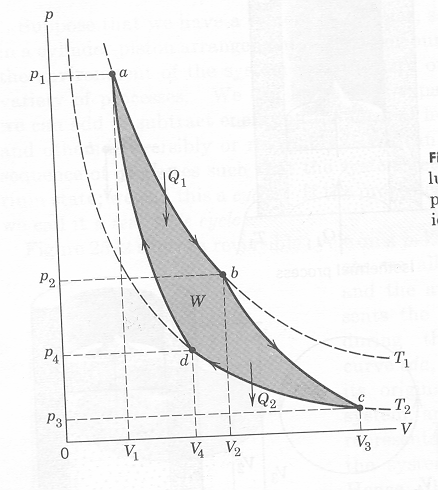
\includegraphics[width=4in]{carnottrim.png}
    \caption{Work as the integrated area of the Carnot cycle}
    \label{fig:carnottrim}
  \end{figure}


But also from (\ref{eq:effic1}) we have:

  \begin{equation}
    \label{eq:cycle2}
\left |  \frac{\Delta q_{in}}{T_1} \right | = \left |  \frac{\Delta q_{out}}{T_2} \right |
  \end{equation}


 

\item This allows us to calculate the efficiency, $\eta$=(work done)/(heat absorbed) as:

  \begin{equation}
    \label{eq:eta}
    \eta=   \frac{ |\Delta q_{in}|- |{\Delta q_{out}}|}{|\Delta q_{in}|}= 1 -\frac{T_2}{T_1}
  \end{equation}
\end{itemize}

So the greater the temperature difference between the Congo and Nova Scotia, the higher the
efficiency of the heat engine.  Taking $T_1$=300 K,$T_2$= 270 K gives and efficiency of about 10\%.

Figure~\ref{fig:carnot2} shows in cartoon form how the system works:

\begin{figure}[htbp]
   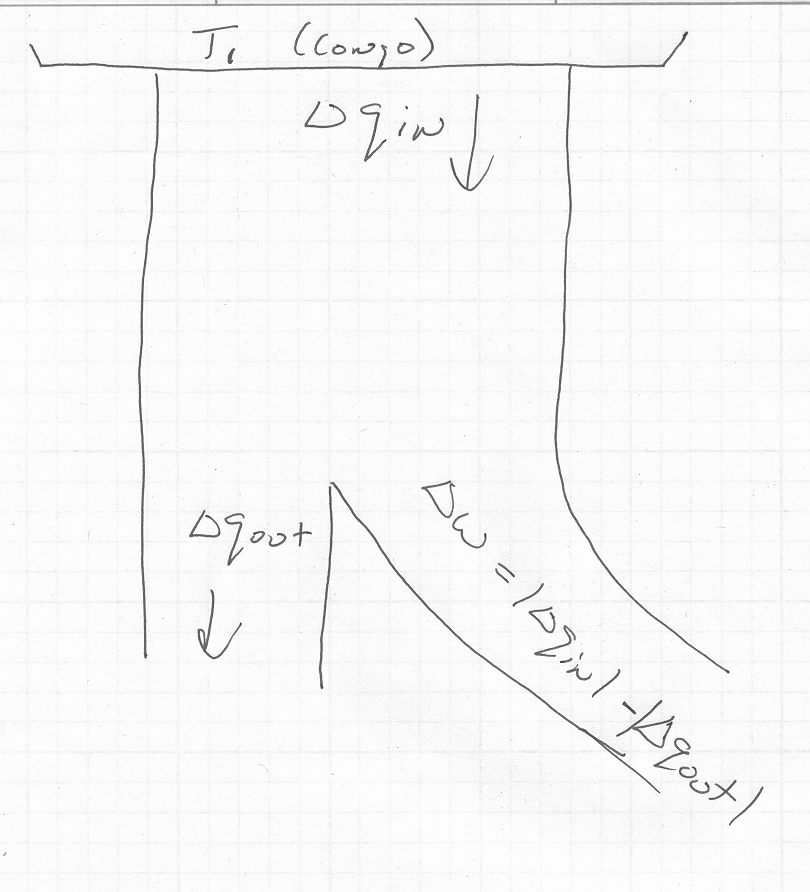
\includegraphics[width=4in]{carnot2.png}  
  \caption{Cartoon of the Carnot cycle}
  \label{fig:carnot2}
\end{figure}

\section{The atmospheric heat engine}
\label{sec:atmosph-heat-engine}

In the atmosphere, we don't typically have isothermal processes.   Note that this equation for the heat engine:


  \begin{equation}
    \label{eq:cycle2}
    \Delta w = | \Delta q_{in} | - | \Delta q_{out} |
  \end{equation}
doesn't depend on an isothermal assumption.  This is where enthalpy is helpful, because from the first law can also be written as:

\begin{equation}
  \label{eq:firsth}
  \frac{dq}{dt} = \frac{dh}{dt} - \alpha \frac{dp}{dt}
\end{equation}
At constant pressure then, we've got:

\begin{equation}
  \label{eq:consp}
  \Delta q = \Delta h
\end{equation}
and this holds for a multiphase system (air, vapor, liquid, ice) just as well as it does for dry air.


\end{document}

%%% Local Variables:
%%% mode: latex
%%% TeX-master: t
%%% End:
